\documentclass[a4paper,10pt, twocolumn]{article}
\usepackage[a4paper,top=2cm,bottom=3cm,left=2cm,right=2cm,footskip=0.8cm]{geometry}
\usepackage{lipsum}
\usepackage{graphicx}
\usepackage{float}
\usepackage{subcaption}
\usepackage{xcolor}
\usepackage{fancyhdr}
\usepackage{helvet}
\usepackage{multicol}
\usepackage{titlesec}     % Para personalizar \section
\usepackage[style=ieee, backend=bibtex, sorting=none, language=portuguese]{biblatex}
\definecolor{grayFEI}{HTML}{7F7F7F}
\usepackage{paracol} % no preâmbulof
\usepackage{indentfirst}  % Indenta o primeiro parágrafo
\setlength{\parindent}{2em}  % Aumenta a indentação para 2em (pode ser ajustado
\titlespacing*{\section}{0pt}{*0}{0pt}
\usepackage{ragged2e}
\usepackage{tikz}
\usepackage{placeins}
\usepackage{caption}
\captionsetup{justification=justified, singlelinecheck=false}

%-------------------------- ESTILOS NÃO ALTERAR ------------------------------------------------%
% Estilo para legendas de figura e tabela
\captionsetup[figure]{
	labelfont={color=azulFEI, bf, small, sf}, % "Figura" azul, negrito, Arial-like
	textfont={small, sf},                    % Texto da legenda em Arial-like
	font=footnotesize,                       % Tamanho aproximado de 9pt
	labelsep=period,                         % "Figura 1." e não "Figura 1:"
	name=Figura,                             % Tradução para "Figura"
	justification=justified,              % Alinhado à esquerda
	singlelinecheck=false                   % Garante alinhamento mesmo em uma linha
}

\captionsetup[table]{
	labelfont={color=azulFEI, bf, small, sf},
	textfont={small, sf},
	font=footnotesize,
	labelsep=period,
	name=Tabela,
	justification=raggedright,
	singlelinecheck=false
}

% Formatação section e subsection
\titleformat{\subsection}
{\color{grayFEI}\normalfont\fontfamily{phv}\selectfont\itshape\fontsize{10}{12}\selectfont}
{\thesubsection.}{0.2em}{}
\renewcommand{\thesubsection}{\Alph{subsection}}

\titleformat{\section}
{\color{azulFEI}\normalfont\fontfamily{phv}\selectfont\bfseries\fontsize{11}{13}\selectfont} % Fonte Helvetica, tamanho 11pt, negrito
{\thesection.}{0.2em}{}
\renewcommand{\thesection}{\Roman{section}} 
\titlespacing*{\section}
{0pt}{10pt}{0pt}

%Formatação Título
\newcommand{\inovatitle}[1]{%
	\noindent{\fontsize{18}{20}{\helvet{\textbf{\textcolor{azulFEI}{#1}}}}}\vspace{25pt}
}

%Formatação Autores
\newcommand{\autores}[1]{
	\helvet{\fontsize{11}{20}\selectfont\textbf{\textit{#1}}}
}
\newcommand{\orientador}[1]{
	\helvet{\fontsize{11}{20}\selectfont\textbf{\textit{#1}}}
}
\newcommand{\filiacao}[1]{
	\helvet{\fontsize{10}{20}\selectfont{\textit{#1}}}
}
\newcommand{\email}[1]{
	\helvet{\fontsize{10}{20}\selectfont{\textit{#1}}\newline}
}
\newcommand{\resumo}[1]{%
	\vspace{15pt}
	\noindent
	{\helvet{\fontsize{12}{20}\selectfont\textbf{\textcolor{azulFEI}{Resumo:}}}} %
	\justifying #1 %
	\newline
}

\newcommand{\keyword}[1]{
	\noindent\helvet{\fontsize{12}{20}\selectfont\textbf{\textcolor{azulFEI}{Palavras-chaves:}}} #1  \vspace{25pt}
}

\renewcommand{\thetable}{\Roman{table}}


% Define a cor azul específica (exemplo: azul FEI)
\definecolor{azulFEI}{HTML}{0070C0} % substitua pelo código que quiser

%Formatação Cabeçalho e rodapé
\setlength{\headsep}{1cm}
\newcommand{\helvet}[1]{{\fontfamily{phv}\selectfont #1}}
\pagestyle{fancy}
\fancyhead{} % limpa cabeçalho
\renewcommand{\headrulewidth}{0.3pt} % ← ATIVA a linha (espessura ajustável)
\setlength\headheight{1.2cm}
\lhead{
\includegraphics[width=4.97cm, height=1cm]{logoinova.png}}
\rhead{\helvet{1º semestre/2025}}

\fancyfoot{} % limpa rodapé
\lfoot{
	\fontfamily{phv}\fontsize{8}{10}\selectfont
	Anais dos Trabalhos de Conclusão de Curso do Centro Universitário FEI, São Bernardo do Campo – SP\\
	\vspace{-4pt}\rule{\textwidth}{1pt} % ← linha abaixo do texto do rodapé
}
\rfoot{\fontfamily{phv}\fontsize{8}{10}\selectfont \thepage}


%-------------------------------- FIM ESTILOS ---------------------------------------------------%



%Adicionar a bibliografia
\addbibresource{referencias.bib}


\begin{document}

\setlength{\columnsep}{20pt}
\twocolumn[%
\begin{@twocolumnfalse}

\raggedright{



\inovatitle{Identificação de melhores momentos em partidas de futebol utilizando sistemas híbridos de visão computacional}


\autores{Lucas Roberto Boccia dos Santos$^1$, Giovanni Chahin Morassi$^1$, Pedro Alexandre Custódio Silva$^1$}

\filiacao{$^1$ Ciência da Computação - campus São Bernardo do Campo}

\email{uniflusantos@fei.edu.br, unifgmorassi@fei.edu.br, unifpesilva@fei.edu.br}

\orientador{Orientador: Murillo Freitas Bouzon}

\filiacao{Departamento de Ciência da Computação, Centro Universitário FEI}

\email{mfbouzon@fei.edu.br}

\resumo{A popularização das plataformas de \textit{streaming} e o consumo dinâmico de mídias digitais impulsionaram drasticamente a demanda por vídeos de "melhores momentos" (\textit{highlights}) em transmissões esportivas. No contexto do futebol, a geração desses recortes é historicamente um processo manual, exaustivo e vulnerável à subjetividade humana, configurando um gargalo operacional crítico. Para mitigar esse problema, a literatura recente converge para a aplicação de técnicas de Visão Computacional. Contudo, soluções puramente espaciais esbarram no desafio da complexidade semântica, falhando em interpretar a intenção tática e a continuidade temporal da jogada. Diante desta lacuna sistêmica, este trabalho propõe o desenvolvimento de uma arquitetura híbrida para a automação de \textit{highlights}, integrando segmentação temporal profunda (TransNet V2), detecção espacial de objetos (YOLO) e classificação semântica multimodal (LLM). Resultados parciais conduzidos sobre o \textit{dataset} SoccerNet-v2 evidenciam a eficácia da ferramenta na delimitação de cenas táticas e sugerem alta estabilidade na detecção de elementos humanos em resolução HD (720p), atingindo confiança mediana de 85\% para jogadores. Em contrapartida, o rastreamento da bola apresentou severa instabilidade (mediana de 48\%), sofrendo achatamento crítico sob degradação extrema de sinal (240p). Estes dados empíricos reforçam as limitações do rastreamento puramente espacial e sustentam a necessidade sistêmica da triagem heurística e da inferência semântica propostas, viabilizando uma solução robusta e escalável para a automação de mídia esportiva.}

\keyword{Visão Computacional, Futebol, Identificação de \textit{Highlights}, Rastreamento de Objetos, YOLO, TransNet V2.}
}

\end{@twocolumnfalse}
]



\section{Introdução}

A indústria do entretenimento esportivo passou por uma transformação radical com o advento do streaming e das plataformas de mídia digital. Diariamente, uma quantidade massiva de conteúdo em vídeo é gerada, transmitida e armazenada globalmente. O futebol, sendo o esporte mais popular do mundo, se encontra no centro dessa transformação \cite{seweryn2026survey}. Nesse cenário de alta disponibilidade e hiperconectividade, o consumo tradicional de partidas completas de noventa minutos divide cada vez mais espaço com formatos de conteúdo mais curtos, dinâmicos e de rápido consumo, alinhados ao ritmo acelerado da sociedade contemporânea \cite{morelli2023fifa, bleier2021survey, deloitte2023sports}.

Dentro da popularização deste formato de consumo, a transmissão de "melhores momentos" (highlights) assume um papel de extremo protagonismo. Clipes que condensam os eventos cruciais de uma partida — como gols, finalizações perigosas e penalidades — são fundamentais para emissoras de televisão, redes sociais e veículos de mídia que buscam maximizar o engajamento de suas audiências. Contudo, a geração de highlights é, historicamente, um gargalo operacional. Trata-se de um processo majoritariamente manual, custoso e exaustivo, que exige o trabalho ininterrupto de editores humanos dedicados a segmentar e classificar os lances em tempo real durante as transmissões, estando também fortemente sujeito à subjetividade \cite{seweryn2026survey, akan2023use}.

A necessidade de escalar a produção de conteúdo esportivo e acelerar a sua disponibilização para o público impulsiona a busca por soluções automatizadas. Para superar as limitações do corte de vídeo manual, torna-se essencial o desenvolvimento de sistemas capazes não apenas de processar o fluxo contínuo de imagens, mas de compreender semanticamente as movimentações e a importância das ações que ocorrem durante uma partida.

Para solucionar o gargalo operacional da edição manual, a literatura tem convergido para a aplicação de técnicas de Visão Computacional e Aprendizado Profundo. Historicamente, a extração de eventos baseava-se em algoritmos de regras manuais e características de baixo nível, como filtros de cor e movimento \cite{seweryn2026survey, akan2023use}. Contudo, a necessidade de capturar interações complexas de alto nível tático impulsionou a adoção de Redes Neurais Convolucionais (CNNs) para o processamento espacial das imagens \cite{akan2023use, xu2025deep}, frequentemente aliadas a Redes Neurais Recorrentes ou arquiteturas baseadas em atenção para a modelagem da continuidade temporal da jogada \cite{yin2024survey, majeed2025real}.

Apesar dos avanços arquiteturais, a análise de partidas de futebol impõe desafios severos que tornam o processo difícil de se lidar, como oclusões constantes entre os atletas, variações de iluminação, desfoque do movimento da bola e qualidade do vídeo \cite{karimi2021soccer, chaganti2024advanced}. O desenvolvimento de modelos robustos contra esses obstáculos só se tornou viável a partir do avanço das técnicas de visão computacional e da consolidação de grandes bases de dados anotadas, com destaque absoluto para o \textit{SoccerNet} e suas variações, que se estabeleceram como o \textit{benchmark} global para tarefas de \textit{action spotting} na comunidade científica \cite{deliege2021soccernet, seweryn2026survey}.

Apoiando-se diretamente na consolidação desses dados, uma vertente robusta da literatura passou a focar primariamente na modelagem da evolução temporal da jogada. O marco preditivo nesse cenário foi estabelecido por Giancola et al. \cite{giancola2018soccernet}, que propuseram a primeira arquitetura de referência (\textit{baseline}) baseada na extração de características visuais temporais. O modelo utilizava recortes de vídeo processados por redes convolucionais 3D para tentar localizar o instante das ações. Embora pioneiro, o sistema original sofria com um campo receptivo temporal limitado, apresentando dificuldades para correlacionar eventos distantes no tempo que culminavam em uma única jogada.

Para mitigar essa limitação temporal e lidar com a imprecisão humana nas marcações de vídeo, a arquitetura evoluiu significativamente com a introdução da Função de Perda Consciente de Contexto (CALF - \textit{Context-Aware Loss Function}) por Cioppa et al. \cite{cioppa2020context}. Diferentemente das abordagens de classificação binária tradicionais, a CALF foi desenhada especificamente para a tarefa de \textit{action spotting}. Ela penaliza a rede de forma branda caso a predição temporal caia nas margens imediatas do evento real, forçando o modelo a aprender a vizinhança contextual da ação (por exemplo, a corrida de um jogador antes do chute em si), e penaliza severamente predições completamente fora do contexto.

Mais recentemente, o estado da arte temporal foi redefinido pela integração de mecanismos de autoatenção baseados em arquiteturas Transformers \cite{zhou2021feature, giancola2025deep}. Essa mudança de paradigma permitiu que as redes abandonassem a análise estritamente sequencial, ponderando matematicamente a relevância de \textit{frames} muito distantes entre si. Essa capacidade de cruzar informações de longo prazo e entender dependências semânticas complexas tornou-se o padrão-ouro nas competições da área \cite{giancola2022soccernet, cioppa2024soccernet}, estabelecendo a base sobre a qual os novos motores de inferência em vídeos esportivos precisam ser construídos.

Em paralelo ao avanço temporal, estudos focados na extração de coordenadas e análise geométrica formam o segundo pilar essencial da literatura. A identificação espacial dos atletas e da bola evoluiu de métodos clássicos \cite{liu2009automatic} para a aplicação de detectores de objetos em tempo real, como o YOLO \cite{redmon2016you, dedgaonkar2025real, darapaneni2022detecting}. Abordagens analíticas modernas passaram a utilizar esses dados de \textit{tracking} aliados a redes convolucionais em grafos (GCN) para classificar interações diretas e a ocupação tática do campo \cite{vidal2022automatic, majeed2025real, indahsari2025implementation}.

\subsection{Bases de Dados em Larga Escala e a Métrica mAP}

A eficácia dessas arquiteturas é intrinsicamente dependente dos dados utilizados. O \textit{SoccerNet} original é composto por 500 partidas completas de campeonatos europeus de elite, anotadas com precisão de um segundo. Em suas iterações mais recentes \cite{giancola2022soccernet, cioppa2024soccernet}, a base foi expandida para incluir milhares de anotações abrangendo classes complexas como faltas, impedimentos e escanteios. No contexto da geração de \textit{highlights}, a tarefa principal é o \textit{Action Spotting}, que exige que o sistema encontre o instante exato em que um evento ocorre dentro de um fluxo contínuo.

Para avaliar matematicamente a precisão de um modelo nessa tarefa, a literatura padronizou o uso da métrica de Precisão Média (\textit{Average Precision} - AP), calculada sob uma janela de tolerância temporal $\delta$. Uma predição temporal $\hat{t}$ é considerada um Verdadeiro Positivo (TP) se existir uma anotação real $t^{*}$ tal que a distância entre elas seja menor ou igual à tolerância $\delta$:
$$ |\hat{t} - t^{*}| \leq \delta $$

Com as definições de Verdadeiros Positivos (TP) e Falsos Positivos (FP) estabelecidas, a métrica final para quantificar o desempenho global do sistema abrangendo todas as classes de eventos é a \textit{mean Average Precision} (mAP), que calcula a área sob a curva de Precisão-Revocação \cite{giancola2022soccernet}:
$$ \mathrm{mAP} = \frac{1}{N} \sum_{c=1}^{N} \mathrm{AP}_{c} $$

A adoção do mAP como função objetivo garante que o sistema não apenas maximize a taxa de acertos brutos, mas mantenha um rigor contra falsos alarmes, um critério inegociável na automação de mídia \cite{cioppa2024soccernet}.

\subsection{Análise Crítica dos Trabalhos Base}

Para fundamentar o desenvolvimento da arquitetura híbrida proposta neste projeto, faz-se necessária uma análise profunda das soluções recentemente propostas pela literatura. A observação crítica do estado da arte permite identificar não apenas as tecnologias consolidadas, mas principalmente as limitações semânticas que ainda persistem na extração autônoma de eventos.

No escopo da automação de análises táticas baseada puramente em visão computacional espacial, o trabalho desenvolvido por Chaganti et al. \cite{chaganti2024advanced} representa um esforço notável para substituir os métodos manuais de coleta de dados físicos. Os autores propuseram uma arquitetura que utiliza o modelo YOLO para a detecção dos atletas em campo. Para garantir a estabilidade da análise frente aos movimentos de câmera (comuns em transmissões esportivas), o sistema incorpora técnicas de fluxo óptico de Lucas-Kanade e utiliza matrizes de homografia para mapear as coordenadas dos pixels para o mundo real. 

Essa conversão dimensional permitiu que o sistema do Chaganti et al. calculasse métricas tangíveis de desempenho, como a distância percorrida e a velocidade em km/h de cada jogador. Contudo, apesar do modelo alcançar impressionantes 98,7\% de precisão no rastreamento de pessoas, o próprio estudo revela uma vulnerabilidade crítica: a detecção da bola obteve apenas 48\% de precisão. Essa falha ocorre devido ao tamanho reduzido do objeto, sua alta velocidade e os constantes momentos de oclusão. Para a geração de \textit{highlights}, onde a bola é o centro gravitacional da ação, depender exclusivamente de um rastreamento espacial tão suscetível a perdas inviabiliza a confiabilidade do sistema, justificando a necessidade de abordagens complementares.

Avançando na tentativa de tornar o rastreamento espacial mais resiliente a essas condições adversas, Indahsari et al. \cite{indahsari2025implementation} exploraram iterações mais recentes de detectores, especificamente avaliando a eficácia do YOLO na automação de decisões de arbitragem (linha de impedimento). O estudo baseou-se em um conjunto de dados expostos a severas variações de iluminação e ângulos de câmera. 

Os resultados de Indahsari et al. provaram que o YOLO (nas variantes Nano e Small) consegue manter uma estabilidade superior na detecção de elementos-chave sob cenários visuais complexos. O estudo reforça a escolha arquitetural do YOLO como um extrator espacial de altíssimo desempenho. No entanto, o escopo da pesquisa focou estritamente em uma análise estática (o instante exato do passe para o impedimento). Sem a incorporação de um motor que avalie a continuidade da jogada, o sistema permanece cego para a evolução tática do lance, resolvendo um problema geométrico isolado, mas não o problema semântico da partida.

Buscando exatamente superar essa barreira semântica e classificar os eventos do jogo de forma contínua, Vidal-Codina et al. \cite{vidal2022automatic} propuseram uma metodologia baseada em algoritmos determinísticos. Utilizando dados de rastreamento 2D já extraídos por provedores comerciais, os autores desenvolveram uma cascata de árvores de decisão. O sistema calcula a distância euclidiana quadro a quadro entre a bola e os atletas, estabelecendo regras de "gatilho" para identificar posses de bola, passes e cruzamentos, alcançando precisão superior a 90\% contra as marcações manuais \cite{vidal2022automatic}.

Embora o trabalho de Vidal-Codina et al. prove que o uso de regras lógicas é um caminho altamente promissor para a classificação de eventos, a sua dependência exclusiva de coordenadas 2D (centros de caixas delimitadoras) o torna estruturalmente frágil em situações de aglomeração. Em lances decisivos, como uma cobrança de escanteio na grande área, a distância entre a bola e o jogador torna-se uma métrica ruidosa. Sem a capacidade de discernir a postura do atleta (saber se o jogador está com a perna estendida para um chute ou apenas correndo próximo à bola), o sistema perde a capacidade de identificar o clímax da jogada de forma confiável.

Por fim, uma vertente distinta da literatura tenta resolver o problema da sumarização esportiva fugindo das limitações do processamento de imagem e apelando para características multimodais. O trabalho de Bez et al. \cite{bez2021multimodal} exemplifica essa abordagem ao focar na alteração do áudio da transmissão. A metodologia desenvolvida baseia-se fortemente na extração do \textit{pitch} (frequência) da voz do narrador, realçado por filtros de pente (\textit{comb-filters}) \cite{bez2021multimodal}. 

Aliando esse dado de áudio a um classificador \textit{Random Forest}, o sistema de Bez et al. processou pequenas janelas temporais de 24 segundos e conseguiu identificar 100\% dos gols em um ambiente de teste, comprimindo partidas inteiras em resumos de poucos minutos. Apesar do êxito numérico, a arquitetura carrega uma falha sistêmica para escalabilidade comercial: a total dependência da narrativa humana. Em eventos transmitidos sem locução (como \textit{feeds} táticos) ou em estádios com ruído excessivo de torcida que mascare a voz do narrador, o modelo entra em colapso. Isso reforça a tese de que a verdadeira autonomia na geração de \textit{highlights} deve derivar da interpretação visual pura das intenções dos atletas.

Essa interpretação visual autônoma, contudo, não pode ser alcançada pelas abordagens espaciais tradicionais. A síntese das limitações da literatura evidencia que o gargalo atual esbarra no desafio da complexidade semântica geométrica. Sistemas baseados apenas em caixas delimitadoras (\textit{bounding boxes}) — cuja aplicação prática é exemplificada na Figura \ref{fig:1} — reduzem o jogador a um bloco rígido. Consequentemente, apresentam severas dificuldades em distinguir a diferença entre um toque irrelevante na bola e um passe crítico, ou entre uma falta tática e uma cobrança de bola parada, pois falham em interpretar a intenção articulada do atleta no contexto da partida \cite{seweryn2026survey, akan2023use}.

\begin{figure*}[htpb] % ← precisa do pacote float
	\centering
	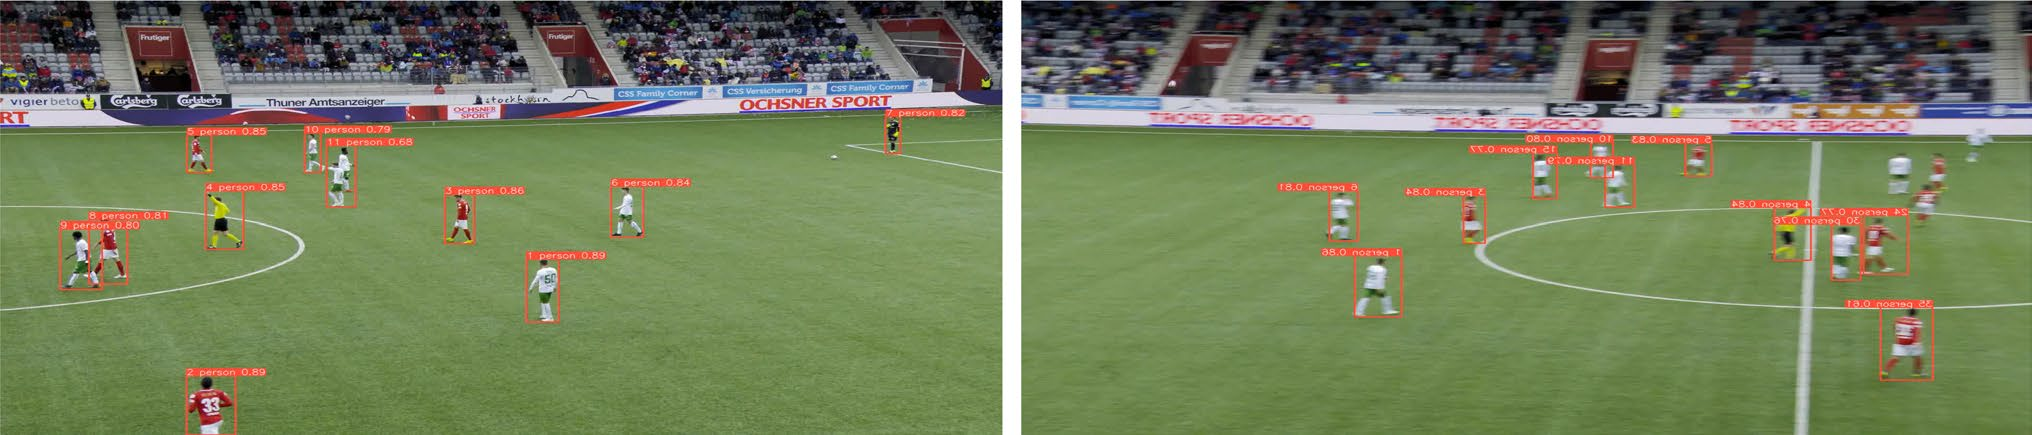
\includegraphics[width=2.0\columnwidth]{player.jpg}
	\caption{Exemplos de extração de características espaciais baseada em modelos de detecção de objetos por caixas delimitadoras (\textit{bounding boxes}) \cite{akan2023use}.}
	\label{fig:1}
\end{figure*}

Para lidar com o problema da segmentação temporal e transições de cena, a literatura tem adotado modelos de redes neurais profundas baseados em convoluções 3D, que processam conjuntamente as dimensões espacial e temporal do fluxo contínuo de vídeo. Nesse contexto, a arquitetura TransNet V2 consolidou-se como uma abordagem no estado da arte para a detecção de transições de cenas \cite{soucek2024transnet, valand2021automated}. O modelo utiliza células convolucionais dilatadas (DDCNN) para extrair características de sequências redimensionadas de quadros. Além da extração de \textit{features} espaciais, a robustez do TransNet V2 baseia-se na incorporação do cálculo de similaridade entre os quadros da sequência, combinando o uso de histogramas de cores RGB com projeções de matrizes de similaridade por cosseno \cite{soucek2024transnet}. Essa arquitetura híbrida permite identificar com alta precisão tanto cortes secos (\textit{hard cuts}) quanto transições graduais complexas (\textit{dissolves}) \cite{soucek2024transnet, valand2021automated, zhu2023autoshot}.

A eficácia geométrica dessa arquitetura de segmentação tem sido explorada e demonstrada especificamente no domínio da mídia esportiva. Valand et al. propuseram um sistema focado no recorte automatizado de melhores momentos no futebol utilizando o TransNet V2 como motor de segmentação de cenas \cite{valand2021automated}. Os autores destacam que os cortes de câmera e transições nas transmissões esportivas costumam ocorrer em sincronia com eventos de alta relevância tática no jogo. Em seu estudo, o modelo foi aplicado diretamente sobre os dados do SoccerNet, extraindo janelas de 100 \textit{frames} para identificar os limites exatos das cenas ao redor de lances críticos, como gols. Os resultados obtidos por Valand et al. demonstraram uma alta precisão na predição das transições, utilizando o modelo pré-treinado do TransNet V2 no contexto futebolístico. Ao aliar essa segmentação profunda com detectores de logotipo de emissoras, os pesquisadores provaram a viabilidade de se estabelecer pontos de ancoragem temporais precisos, servindo de base sólida para a construção de fluxos de trabalho autônomos na sumarização de partidas \cite{valand2021automated}.

\begin{figure}[htpb] % ← precisa do pacote float
	\centering
	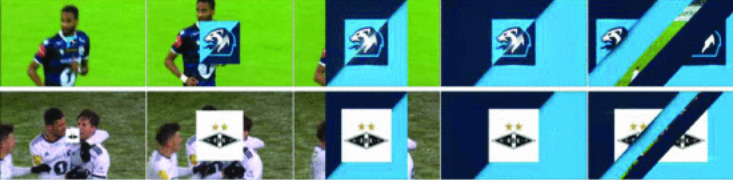
\includegraphics[width=1.0\columnwidth]{transnetv2.jpg}
	\caption{Exemplo de utilização do TransNet V2 para a obtenção de cortes de cena em uma partida de futebol. Cada imagem representa um corte de câmera diferente em uma transmissão de futebol \cite{valand2021automated}.}
	\label{fig:2}
\end{figure} 

Diante dessa lacuna, a detecção automática de melhores momentos exige abordagens híbridas que consigam fundir a percepção espacial do campo com a lógica temporal da jogada \cite{xarles2023astra}. Portanto, o objetivo central deste trabalho é desenvolver um sistema híbrido de Visão Computacional que interprete ativamente a semântica da cena e culmine no recorte temporal preciso e automatizado dos instantes mais relevantes da partida.

\section{Metodologia}

A arquitetura proposta para a automação da geração de \textit{highlights} fundamenta-se em um pipeline de processamento híbrido, que integra técnicas de segmentação temporal, detecção de objetos e inferência semântica profunda. O fluxo de trabalho é desenhado para converter o vídeo bruto em metadados estruturados, otimizando o processo de geração e sua confiabilidade por meio de filtragens sucessivas. A Figura \ref{fig:3} demonstra o fluxograma pretendido para a execução do projeto.

\begin{figure*}[htpb] % ← precisa do pacote float
	\centering
	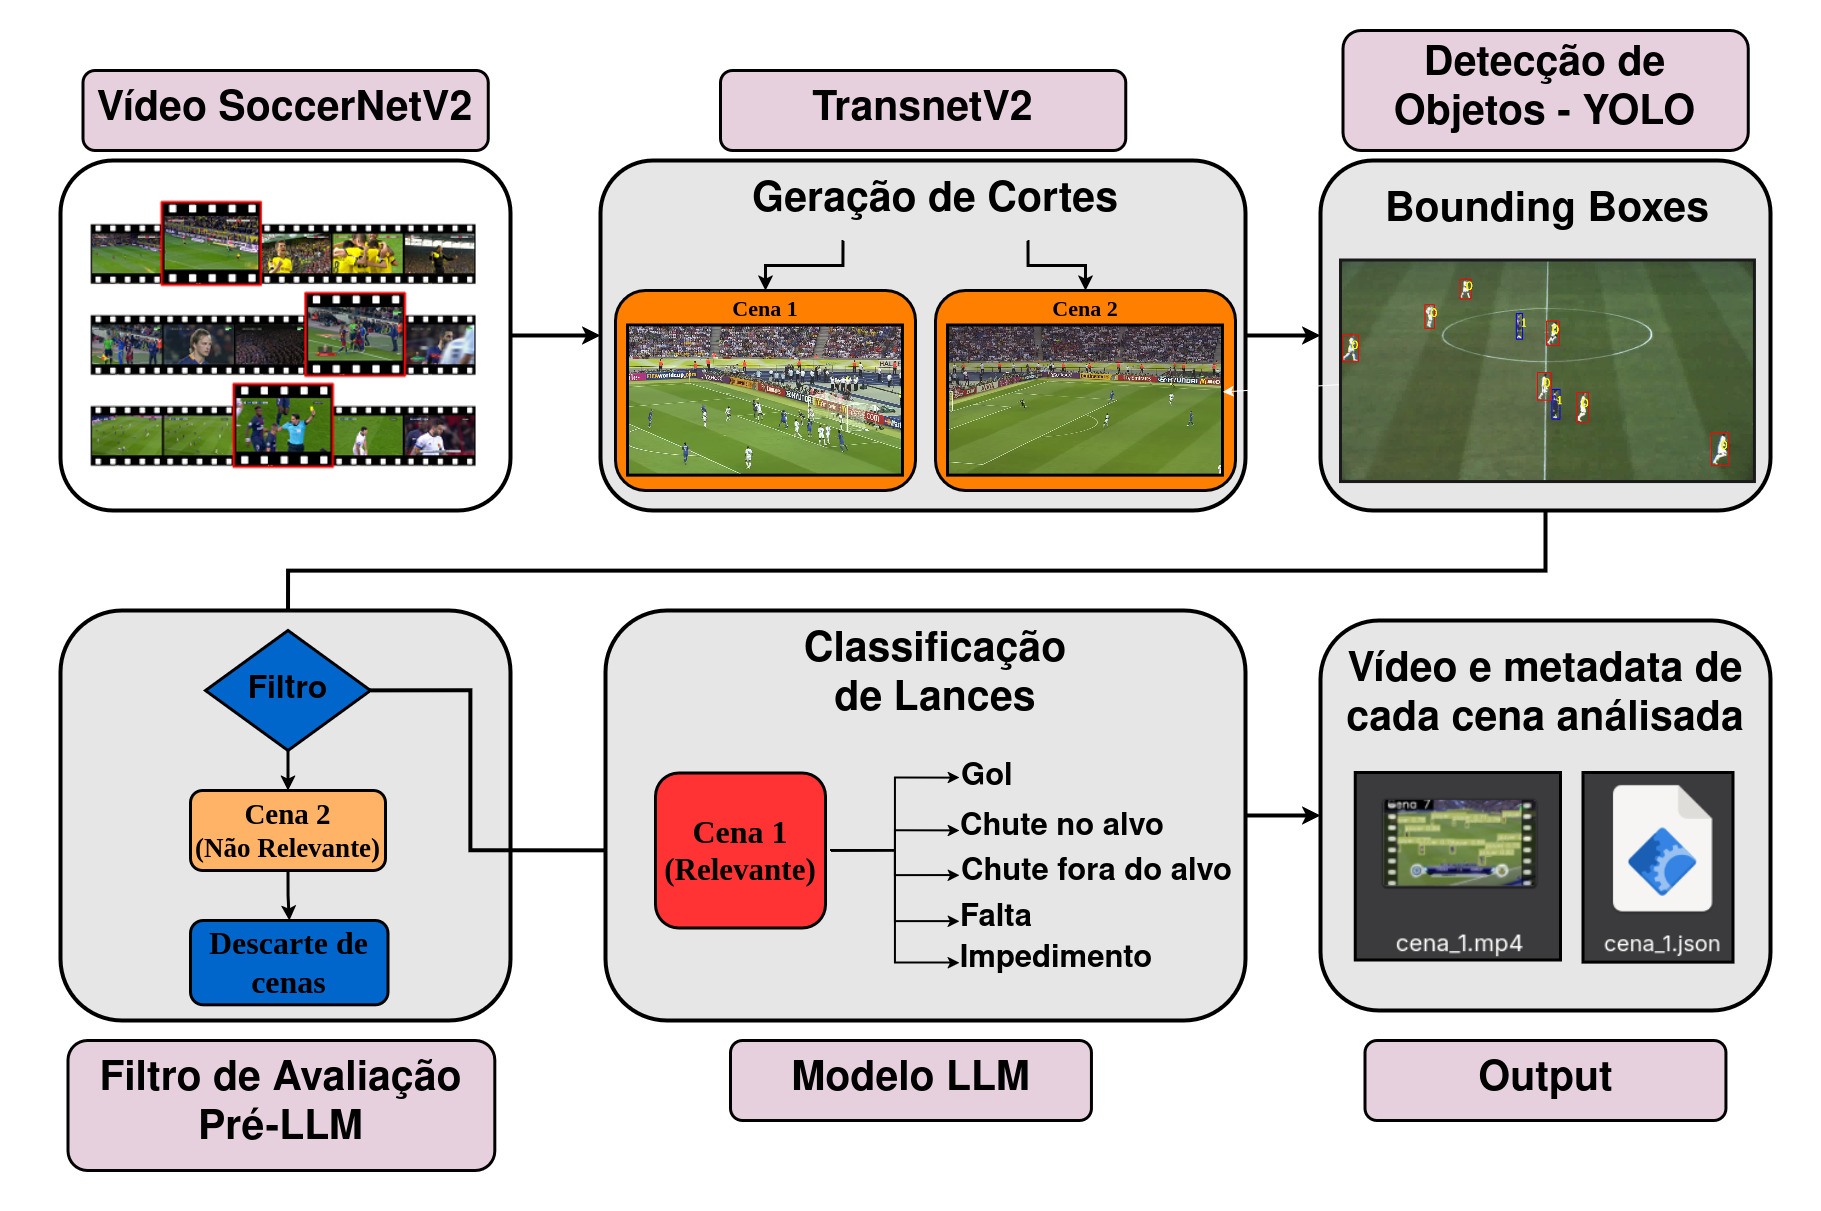
\includegraphics[width=1.75\columnwidth]{b.jpg}
	\caption{Fluxograma da arquitetura híbrida proposta para a automação de melhores momentos: segmentação temporal (TransNet V2), detecção espacial (YOLOv8), triagem de relevância (Filtro Pré-LLM) e classificação semântica (Modelo LLM). As imagens ilustrativas do arquivo de entrada e do processo de detecção de objetos foram adaptados de Giancola \textit{et. al} \cite{giancola2018soccernet} e Hanzra e Rossi \cite{hanzra2013automatic}, respectivamente. O exemplo visual da geração de cortes de cena é uma reprodução do canal FIFA no YouTube e as classes de lances baseiam-se em Zhou \textit{et al.} \cite{zhou2021feature}.}
	\label{fig:3}
\end{figure*}

Ao fragmentar a partida original em unidades temporais contínuas e delimitadas, a segmentação de cenas atua como o alicerce metodológico para o sistema híbrido proposto, conforme estruturado no fluxograma da Figura 3. O processamento inicial pelo TransNet V2 elimina a redundância computacional em quadros de transição e prepara o ambiente visual para que o modelo espacial (YOLOv8) rastreie as entidades-chave de forma isolada. Dessa forma, a arquitetura proposta visa superar a cegueira semântica das abordagens tradicionais filtrando o volume de dados e fornecendo fragmentos altamente qualificados para a interpretação final por Modelos de Linguagem Multimodais, culminando na detecção e recorte autônomo dos instantes mais relevantes da partida.


\subsection{Aquisição e Segmentação Temporal (TransNet V2)}

O sistema utiliza como entrada primária o \textit{dataset} SoccerNet-v2 \cite{deliege2021soccernet}, que fornece vídeos de transmissões televisivas de partidas de futebol. Devido à natureza contínua do fluxo de vídeo, a primeira etapa crítica consiste na segmentação temporal. Para este fim, emprega-se o modelo TransNet V2, uma rede neural convolucional profunda especializada na detecção de limites de cenas (\textit{shot boundary detection}). 

O TransNet V2 identifica cortes de câmera e transições abruptas, fragmentando a partida em um conjunto discreto de cenas $C = \{c_1, c_2, \dots, c_n\}$, como o mostrado na Figura 2. Esta etapa é vital para garantir que os módulos subsequentes operem sobre contextos visuais semanticamente coerentes, eliminando a redundância de processamento entre quadros de transição ou replays.

\subsection{Detecção Espacial e Criação de Bounding Boxes (YOLO)}

Sobre as cenas individualizadas, aplica-se o modelo YOLOv8 (\textit{You Only Look Once}) para a extração de características espaciais em tempo real. O detector é configurado para a identificação de quatro classes de entidades fundamentais: jogadores de linha, goleiro, árbitro e a bola de futebol. 

A escolha do YOLOv8 justifica-se pela sua eficiência comprovada na detecção de objetos, incluindo em partidas de futebol, conforme sugerido pela literatura recente \cite{indahsari2025implementation, dedgaonkar2025real, redmon2016you}. O \textit{output} desta etapa consiste na geração de caixas delimitadoras (\textit{bounding boxes}) que fornecem a posição relativa (x, y) de cada entidade no campo de visão, servindo como base geométrica para o entendimento do contexto do lance.

\subsection{Triagem Contextual e Filtro Pré-LLM}

Dado o alto custo computacional da inferência em modelos de linguagem de larga escala, introduz-se uma camada de triagem heurística Pré-LLM. Este módulo atua como um filtro de relevância baseado em contexto espacial, operando sobre o vídeo com as \textit{bounding boxes} geradas pela aplicação do YOLOv8.

Cenas que apresentam baixa atividade tática — como bola fora de jogo, substituições ou foco exclusivo na torcida — são classificadas como "Não Relevantes" e descartadas. A lógica de filtragem prioriza cenas onde há uma convergência de múltiplos atletas em zonas críticas ou alta velocidade de deslocamento da bola, garantindo que apenas lances com alta probabilidade de serem \textit{highlights} sejam encaminhados para a análise semântica do modelo LLM.

\subsection{Classificação Semântica via Modelos de Linguagem (LLM)}

\begin{figure*}[t!] % ← precisa do pacote float
	\centering
	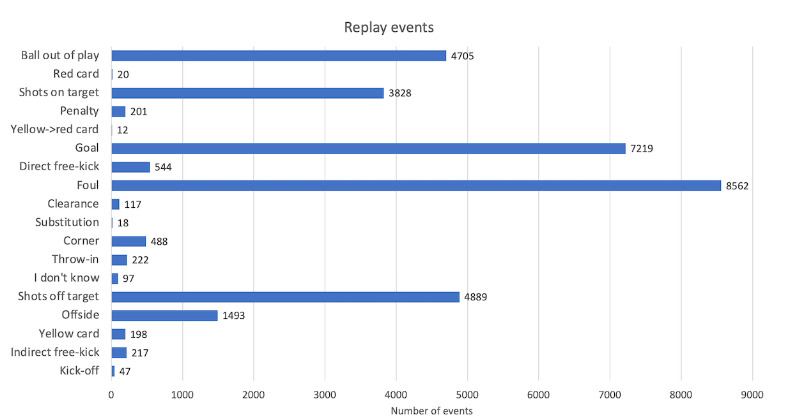
\includegraphics[width=2.0\columnwidth]{baidu.jpg}
	\caption{Distribuição quantitativa das classes de eventos mapeadas no \textit{dataset} SoccerNet-v2. Adaptado de Zhou \textit{et al.} \cite{zhou2021feature}.}
	\label{fig:4}
\end{figure*}

As cenas selecionadas são processadas por um \textit{Large Language Model} com capacidades multimodais. Nesta etapa, o sistema realiza a transição do dado puramente visual para o entendimento semântico do esporte. O modelo é instruído a classificar o lance em categorias predefinidas, representando eventos da partida.

A seleção das categorias baseia-se no estudo de Zhou \textit{et al.} \cite{zhou2021feature}, que analisou os vídeos do \textit{dataset SoccerNet-v2} e mapeou a frequência de ocorrência de diversos eventos de jogo. A Figura \ref{fig:4} ilustra a distribuição quantitativa desses eventos, conforme reportado pelos autores.

A partir dos dados apresentados na Figura \ref{fig:4}, foram selecionados para este trabalho os cinco eventos de maior incidência que representam potenciais \textit{highlights} (lances de destaque). A situação \textit{ball out of play} (bola fora de jogo), embora figure como o quarto evento mais frequente, foi excluída por não configurar uma jogada de interesse para a composição de um compilado de \textit{highlights}. Dessa forma, as cinco categorias finais estabelecidas são: Gol (momento máximo do esporte, conclusão bem-sucedida de uma jogada que resulta em alteração no placar); Chute no alvo (finalização direcionada aos limites da meta que é defendida ou bloqueada); Chute fora do alvo (finalização que não atinge os limites da meta); Falta (interrupção do jogo decorrente de infração); e Impedimento (infração de posicionamento detectada pela arbitragem).

\subsection{Estrutura de Saída e Persistência de Dados}

O output do sistema consiste no arquivo de vídeo original da cena analisada, cortada anteriormente pelo \textit{TransNet V2}, junto de um arquivo .json com o metadata da análise, contendo os detalhes da detecção de highlights, incluindo o \textit{timestamp} em que o(s) \textit{highlight(s)} ocorre dentro do vídeo, a classificação dos mesmos dentro das categorias mencionadas anteriormente e um identificador particular do \textit{highlight} para a cena analisada.

\section{Resultados Parciais}

O desenvolvimento da arquitetura híbrida proposta encontra-se em fase de testes de integração, com os módulos de segmentação temporal e extração espacial já operacionais. Os experimentos preliminares foram conduzidos utilizando fragmentos de vídeo extraídos do \textit{dataset} SoccerNet-v2, permitindo avaliar o comportamento isolado dos modelos TransNet V2 e YOLOv8 antes da aplicação do filtro heurístico e do processamento semântico via LLM.

\subsection{Segmentação Temporal e Extração de Cenas}

Na primeira etapa do \textit{pipeline}, o modelo TransNet V2 foi aplicado sobre o fluxo de vídeo bruto para realizar a detecção de transições de cena (\textit{shot boundary detection}). O modelo demonstrou capacidade de fragmentar o vídeo contínuo em unidades semânticas discretas. 

A Figura \ref{fig:exemplo_cenas_limpas} ilustra dois exemplos de cenas individualizadas pelo modelo (Cenas 8 e 9). A precisão do corte temporal permitiu isolar fragmentos focados na reação dos atletas após lances capitais. Esta etapa inicial confirmou-se essencial para reduzir a carga computacional subsequente, delimitando contextos visuais coerentes e eliminando replays e transições ruidosas da transmissão original.

\begin{figure*}[htpb]
	\centering
	% Cena 8
	\begin{subfigure}[b]{0.48\textwidth}
		\centering
		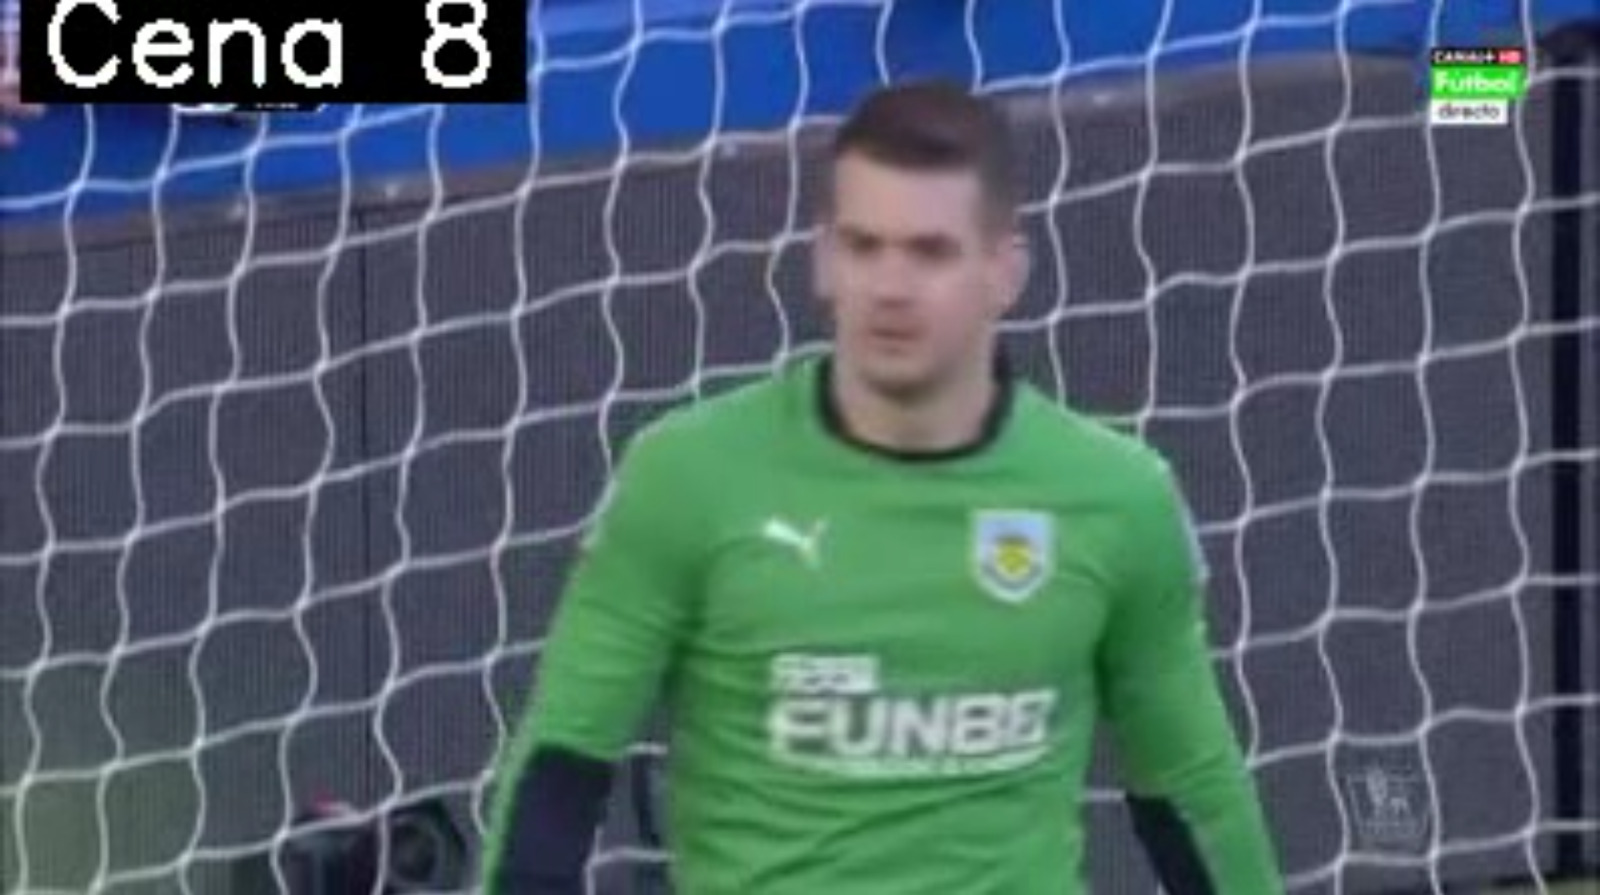
\includegraphics[width=\textwidth]{cena8.jpg} % Nome do arquivo da Cena 8
		\caption{Exemplo da "Cena 8" extraída pelo TransNet V2.}
		\label{fig:cena8}
	\end{subfigure}
	\hfill
	% Cena 9
	\begin{subfigure}[b]{0.48\textwidth}
		\centering
		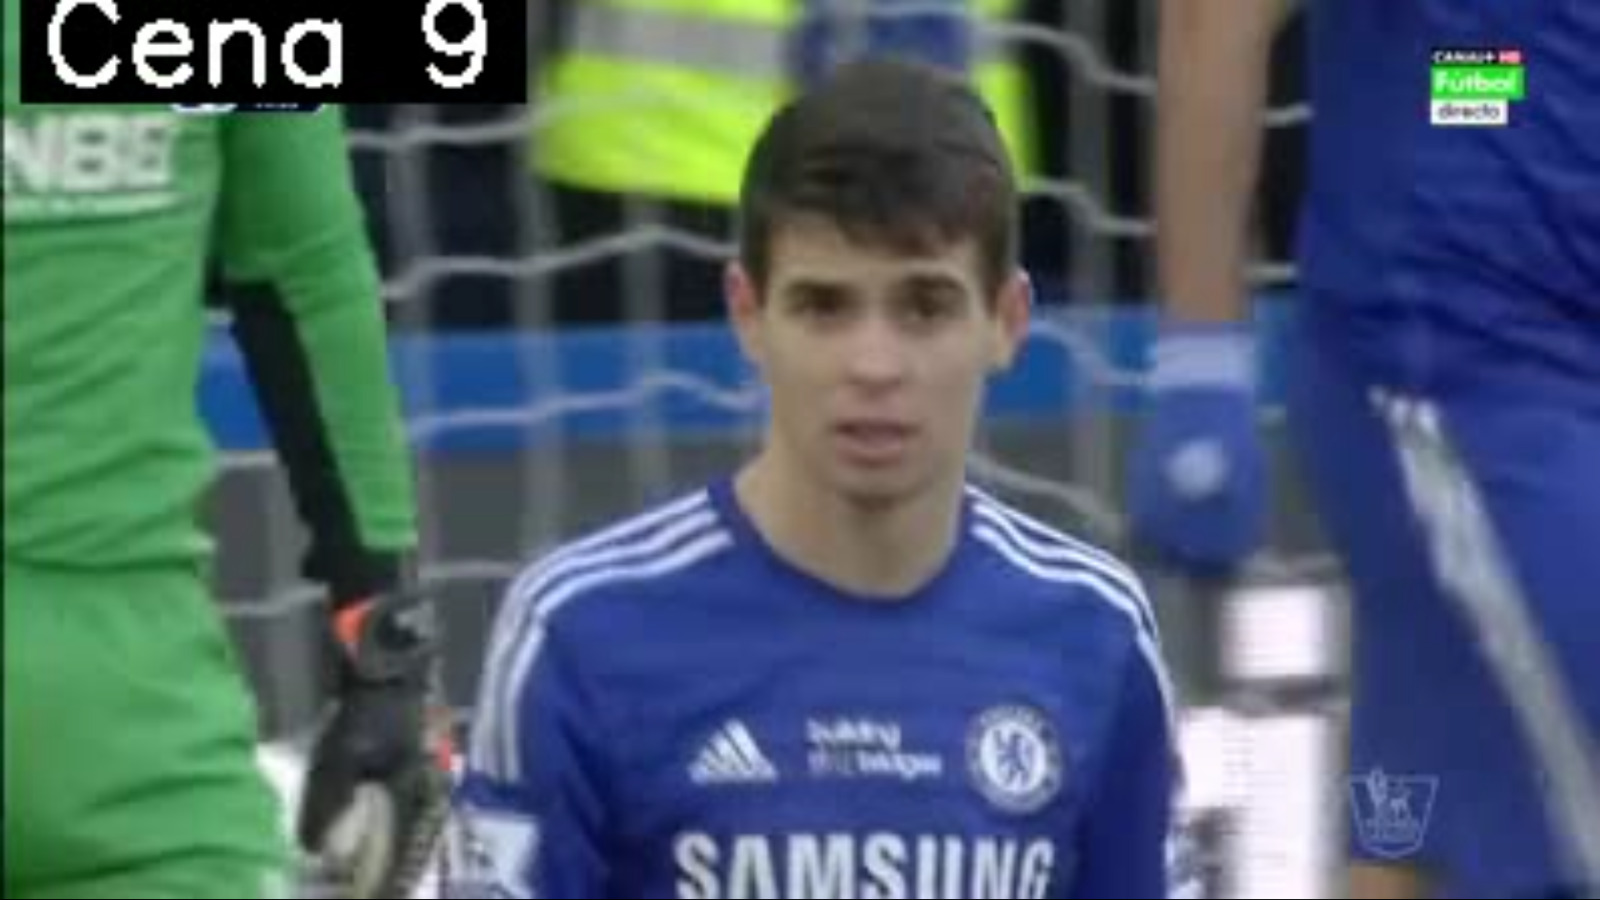
\includegraphics[width=\textwidth]{cena9.jpg} % Nome do arquivo da Cena 9
		\caption{Exemplo da "Cena 9" extraída pelo TransNet V2.}
		\label{fig:cena9}
	\end{subfigure}
	
	% Legenda Unificada e Rigorosa
	\caption{Exemplos de cenas individualizadas temporalmente pelo modelo TransNet V2. As imagens ilustram a saída visual do \textit{pipeline} integrado. A ausência de sobreposições de detecção (\textit{bounding boxes}) decorre da execução subsequente do modelo YOLOv8 sobre enquadramentos de close-up extremo, que descaracterizam a geometria corporal padrão das classes treinadas.}
	\label{fig:exemplo_cenas_limpas}
\end{figure*}

\subsection{Desempenho da Detecção Espacial (YOLO)}

As cenas individualizadas foram submetidas ao modelo YOLOv8 para a identificação espacial e contínua das entidades fundamentais do jogo (jogador, árbitro, bola, goleiro). A Figura \ref{fig:yolo_image} apresenta o resultado visual da aplicação bem-sucedida das \textit{bounding boxes} por parte do YOLO sobre um quadro tático de plano aberto (Cena 10) cortado pelo TransNet V2.

\begin{figure}[h!]
	\centering
	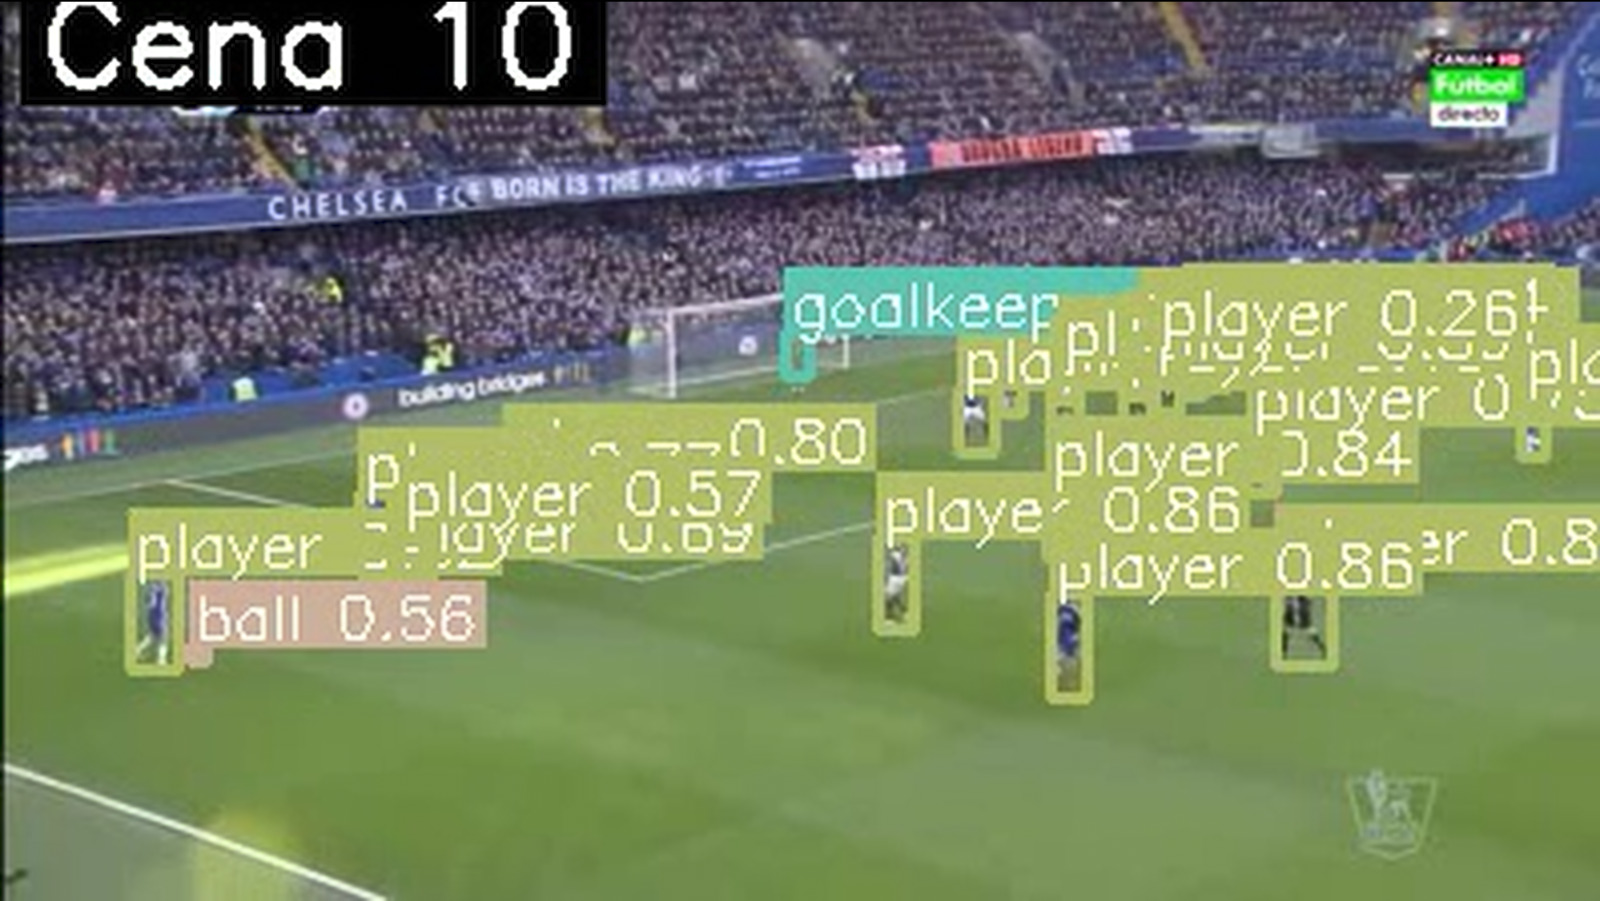
\includegraphics[width=1\columnwidth]{yolo_image.jpg}
	\caption{Aplicação das \textit{bounding boxes} por parte do YOLOv8 sobre um quadro tático (Cena 10) cortado pelo TransNet V2.}
	\label{fig:yolo_image}
\end{figure}

A inferência principal foi conduzida em resolução HD (720p), alinhada aos padrões mínimos de transmissão esportiva atual. Para quantificar o desempenho preliminar, adotou-se como métrica o Nível de Confiança Médio (\textit{Average Confidence Score}) ao longo dos quadros analisados, cuja dispersão e variabilidade para cada classe detectada podem ser observadas na Figura \ref{fig:dispersao_yolo}.

\begin{figure}[h!]
	\centering
	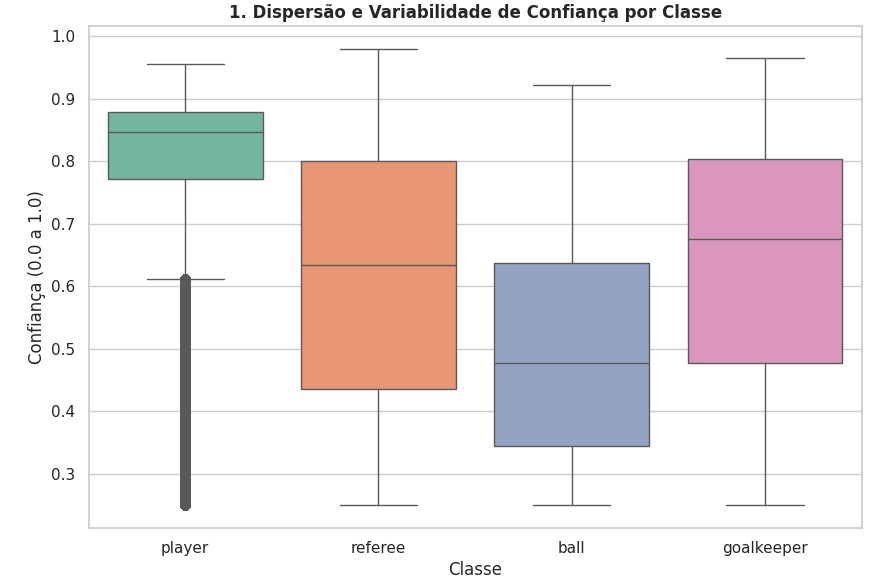
\includegraphics[width=1\columnwidth]{yolo.jpg} % Nome do arquivo do Boxplot
	\caption{Dispersão e variabilidade do nível de confiança das predições do YOLOv8 (720p) categorizadas por classe de objeto detectado.}
	\label{fig:dispersao_yolo}
\end{figure}

A análise quantitativa extraída dessa distribuição sugere uma estabilidade notável na detecção de elementos humanos. O modelo sustentou um nível de confiança mediano de 85\% para a classe de jogadores de linha (box plot \textit{player}). A diferenciação de indivíduos com base no vestuário também se mostrou robusta, com a classe dos goleiros registrando 68\% de confiança (box plot \textit{goalkeeper}) e a dos árbitros, 63\% (box plot \textit{referee}). 

Contudo, corroborando os desafios descritos na literatura, o rastreamento da bola de futebol apresentou índices de confiança consideravelmente mais oscilantes, com mediana de 48\%. Conforme evidenciado pela amplitude da caixa representativa da classe \textit{ball} na figura, essa instabilidade deve-se à rápida movimentação do objeto, ao desfoque de movimento (\textit{motion blur}) e às oclusões constantes geradas pelos corpos dos atletas.

\subsection{Impacto da Degradação do Sinal de Vídeo}

Para avaliar a resiliência geométrica do modelo à degradação do sinal de vídeo e testar os limites da extração puramente espacial, a mesma inferência foi executada sobre os quadros reamostrados para a resolução de 240p.

Como esperado pela fundamentação teórica de redes convolucionais, a subamostragem severa de pixels impactou criticamente a detecção de objetos em pequena escala. A Figura \ref{fig:dispersao_240p} ilustra a queda generalizada nos níveis de confiança.  Enquanto a identificação de jogadores sofreu uma deterioração estrutural no seu limite inferior (com o surgimento de múltiplos \textit{outliers} de baixa confiança na distribuição) e a mediana recuou de 85\% para 81\%, a detecção da bola sofreu um achatamento severo, com a mediana caindo para 44\%. Em 240p, a bola reduz-se a uma área de pouquíssimos pixels, fundindo-se com o ruído de fundo do gramado. 

\begin{figure}[h!]
	\centering
	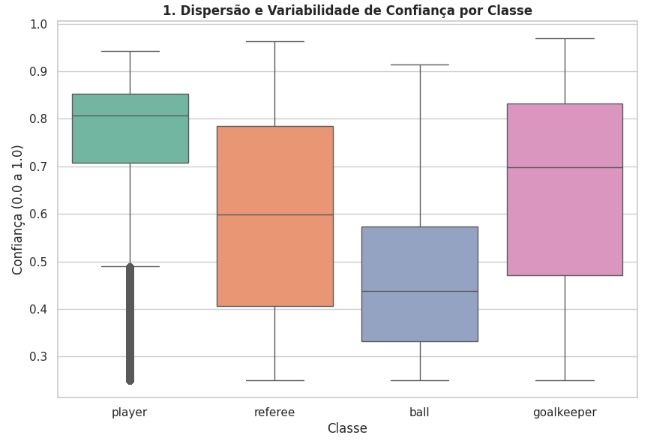
\includegraphics[width=1\columnwidth]{yolo240p.jpg}
	\caption{Dispersão e variabilidade do nível de confiança das predições do YOLOv8 em cenário de degradação extrema (240p), evidenciando o achatamento da confiança na classe da bola.}
	\label{fig:dispersao_240p}
\end{figure}

Estes resultados parciais reforçam categoricamente a necessidade da arquitetura híbrida proposta. A fragilidade do rastreamento puramente espacial (especialmente em condições visuais adversas) evidencia que a adoção do Filtro Pré-LLM e da classificação semântica temporal não são apenas melhorias marginais, mas sim requisitos sistêmicos para a automação confiável de \textit{highlights}.

\subsection{Avaliação dos Modelos Multimodais (LLM)}

Para validar a etapa semântica da arquitetura, foi desenvolvido um \textit{benchmark} local sobre segmentos extraídos do \textit{dataset} SoccerNet-v2. Cada segmento foi enviado a um modelo multimodal com uma instrução fixa para produzir uma resposta JSON estruturada contendo o tipo do segmento, a classe do evento, o instante relativo do lance e a confiança da predição. Como a avaliação dos LLMs foi conduzida sobre respostas estruturadas por segmento, adotamos F1 com janela temporal de 5 segundos (F1@5s), precisão, revocação, acurácia do tipo de segmento e taxa de saída válida, em vez do mAP tradicional utilizado em competições de \textit{action spotting}. Dessa forma, a métrica avalia simultaneamente a localização temporal do evento e a viabilidade prática do modelo dentro de um sistema automatizado.

Inicialmente, foram executados testes de triagem com amostras pequenas para avaliar a compatibilidade operacional dos modelos. Estes testes não tinham como objetivo comparar desempenho final, mas verificar se cada modelo conseguia satisfazer os requisitos mínimos: aceitar vídeo como entrada, retornar JSON no formato exigido e produzir uma predição semanticamente interpretável. A Tabela \ref{tab:llm_triagem} mostra que apenas parte dos modelos avaliados conseguiu manter saídas válidas de forma consistente, evidenciando que a confiabilidade estrutural da resposta é um critério tão importante quanto a precisão pontual.

\begin{table*}[t!]
	\centering
	\caption{Triagem dos modelos multimodais avaliados quanto à capacidade de processar vídeo e produzir a saída estruturada exigida pelo sistema.}
	\label{tab:llm_triagem}
	\resizebox{\textwidth}{!}{%
		\begin{tabular}{|l|c|c|c|l|}
			\hline
			\textbf{Modelo} & \textbf{Segmentos} & \textbf{Saídas válidas} & \textbf{F1@5s} & \textbf{Observação} \\ \hline
			\texttt{google/gemini-3.1-flash-lite} & 30 & 100,0\% & 0,597 & Melhor equilíbrio preliminar entre validade e F1. \\ \hline
			\texttt{qwen/qwen3.6-plus} & 30 & 93,3\% & 0,474 & Alta taxa de validade, com F1 inferior ao Gemini 3.1 Flash Lite. \\ \hline
			\texttt{google/gemini-3.5-flash} & 30 & 33,3\% & 0,357 & Precisão alta, mas baixa confiabilidade estrutural. \\ \hline
			\texttt{perceptron/perceptron-mk1} & 30 & 0,0\% & 0,000 & Não satisfez o formato estruturado de saída na amostra de triagem. \\ \hline
			\texttt{qwen/qwen3.6-flash} & 30 & 0,0\% & 0,000 & Não satisfez o formato estruturado de saída na amostra de triagem. \\ \hline
			\texttt{google/gemma-4-26b-a4b-it:free} & 1 & 0,0\% & 0,000 & Falhou no teste inicial de saída estruturada. \\ \hline
			\texttt{google/gemma-4-31b-it:free} & 1 & 0,0\% & 0,000 & Falhou no teste inicial de saída estruturada. \\ \hline
			\texttt{google/gemma-4-31b-it} & 1 & 100,0\% & 0,000 & Produziu saída válida, mas sem evidência suficiente de desempenho. \\ \hline
			\texttt{google/gemini-3.1-pro-preview} & 1 & 0,0\% & 0,000 & Falhou no teste inicial de saída estruturada. \\ \hline
			\texttt{xiaomi/mimo-v2.5} & 1 & 0,0\% & 0,000 & Falhou no teste inicial de saída estruturada. \\ \hline
			\texttt{z-ai/glm-5v-turbo} & 1 & 0,0\% & 0,000 & Falhou no teste inicial de saída estruturada. \\ \hline
		\end{tabular}%
	}
\end{table*}

A partir dessa triagem, foram selecionados para a avaliação ampliada os três modelos que apresentaram a melhor combinação entre taxa de respostas válidas e desempenho preliminar: \texttt{google/gemini-3.1-flash-lite}, \texttt{google/gemini-3.5-flash} e \texttt{qwen/qwen3.6-plus}. A comparação final foi conduzida sobre a mesma seleção compartilhada de 1000 segmentos, garantindo que todos os modelos fossem avaliados exatamente sobre os mesmos exemplos. Essa decisão controla a variação da amostra e torna a diferença entre os modelos atribuível ao comportamento de inferência, não à dificuldade relativa dos segmentos avaliados.

\begin{table*}[t!]
	\centering
	\caption{Comparação dos três modelos selecionados em 1000 segmentos compartilhados do SoccerNet-v2, utilizando janela temporal de 5 segundos.}
	\label{tab:llm_benchmark_final}
	\resizebox{\textwidth}{!}{%
		\begin{tabular}{|l|c|c|c|c|c|c|c|c|}
			\hline
			\textbf{Modelo} & \textbf{Saídas válidas} & \textbf{Precisão} & \textbf{Revocação} & \textbf{F1@5s} & \textbf{Tipo segmento} & \textbf{Custo (US\$)} & \textbf{Latência média} & \textbf{Saídas inválidas} \\ \hline
			\texttt{google/gemini-3.1-flash-lite} & 100,0\% & 0,648 & 0,551 & 0,596 & 0,566 & 1,287 & 5,59s & 0 \\ \hline
			\texttt{google/gemini-3.5-flash} & 56,8\% & 0,787 & 0,390 & 0,521 & 0,651 & 7,251 & 4,72s & 432 \\ \hline
			\texttt{qwen/qwen3.6-plus} & 98,2\% & 0,437 & 0,355 & 0,392 & 0,509 & 1,465 & 9,04s & 18 \\ \hline
		\end{tabular}%
	}
\end{table*}

\section{Referências}
\printbibliography[heading=none]

\end{document}